\documentclass[twocolumn]{article}
\usepackage{graphics}
\usepackage{graphicx}
\usepackage[utf8]{inputenc}
\usepackage{hyperref}
\usepackage{natbib}

\newcommand{\aetitle}{Algorithm Engineering Report 01} % Title of the report
\newcommand{\studentOne}{Patrick Koston} % Name 1
\newcommand{\studentTwo}{Simon Schwitz} % Name 2


\begin{document}

\twocolumn[{\begin{small}
\begin{minipage}{0.5 \linewidth}
  Algorithm Engineering\\
  WS 23/24
\end{minipage}
\begin{minipage}{0.5\linewidth}
  \begin{flushright}
    \studentOne\\
    \studentTwo
  \end{flushright}
\end{minipage}
\end{small}}
{\begin{center}
\begin{sffamily}\Large\bfseries \aetitle \end{sffamily}
\end{center}}
\vskip 3em]

\begin{abstract}
    The abstract gives a short summary of the project. Begin by stating the motivation of the research at hand, describe the problem and shortly describe what methods you used to solve this problem. Finally, name the most important findings and provide a brief conclusion of your work.
\end{abstract}


\section{Introduction}
Trying to go through files and order elements in them is a task we're often faced with, to do it in an optimal way on our system. But problems arise, if our system can't handle the files it's trying to sort, mostly in terms of the size of the file and how to read all of it into the RAM (\textbf{R}andom \textbf{A}ccess \textbf{M}emory), much less work on the input in RAM.\\
For this, we want to focus this report on an algorithm that can work to sort in such an scenario, go over its implementation and show the results of it running on our devices.

\section{Preliminaries}
%Theoretical Knowledge applied here
%The algorithm we are wanting to focus on is External Memory MergeSort, or short EM-MergeSort.
%For the task of sorting data entries we are focusing on MergeSort. It functions by firstly dividing all entries into singular entries, then merging them together into parts and sorting them during that process. With this, we can work on smaller arrays of objects.
The main algorithm for this project is going to be External MergeSort.\\
MergeSort function through the concept of "divide \& conquer", as is usual with sorting algorithms. It first divides all entries into blocks, only containing the entry itself. Then, through comparing two blocks, it sorts the two entries and inserts it into a new block, which is the combination of the two previous blocks.\\
This process repeats until only one block remains, which contains an ordered list of all entries.\\
%For our project, we want to utilize the external memory model, so that we can work on files that are larger in size than the RAM unit utilized in our system, since we don't want to load all entries into it at once. The basis for this is to look at the memory available or space used as blocks filling the memory of the external and internal memory. 
To continue, we need to define the External Memory (EM) model, which is the basis for the used algorithm. For it, we use an internal memory of size \textit{M}, which will be used to read our input file of size $N$. We define blocks that can be loaded into memory with size \textit{B}, which is much less than \textit{M}. 
Furthermore, we can distinguish between the number of data blocks in the input file, which is defined as $n = \lceil \frac{N}{B}\rceil$, as well as the number of blocks that can be loaded into memory, defined as $m = \lfloor \frac{M}{B}\rfloor$.


\section{Algorithm \& Implementation}
%This section provides information about the actually used algorithms and their respective implementations. It should roughly cover the following three topics:
%\begin{itemize}
%	\item \textbf{Advanced Algorithm:}\\
%		Give and explain the advanced algorithms that you used, and compare them to the basic algorithms.
%	\item \textbf{Implementation:}\\
%		Explain how you implemented these algorithms and state what external libraries you used.
%	\item \textbf{Algorithm Engineering Concepts:}\\
%		State the algorithm engineering concepts that you used and explain why they were helpful (if applicable).
%\end{itemize}

External MergeSort functions through the following steps:
\begin{itemize}
	\item \textbf{Partitioning:}\\
	Data entries are split into blocks of a defined size \textit{B}. Of these blocks, \textit{m} blocks are loaded into memory and are initially sorted inside their blocks. This is repeated until all blocks have been considered, sorted and written back to external memory.
	\item \textbf{Merging:}\\
	Two blocks are loaded into internal memory. In addition to these two blocks, one buffer in the size of a block is defined in internal memory. We then work with pointers to their respective data in the buffer and compare them. The smaller value is written into the buffer and the pointer of the block which value was written gets moved one position farther. Once the buffer is full, it is flushed into external memory, so that sorting in the remaining blocks can continue without complications. Once a block to be sorted is cleared, it is removed from internal memory and another block is loaded to be compared and sorted with the remaining block. This process is repeated until all consecutively defined blocks are run through. Then, this whole process is repeated until only one block remains.\\
	An alternative to this approach is by utilizing the internal memory more effectively is \textit{k}-way Merging, which describes running \textit{k} blocks inside of internal memory at once. \textit{k} is defined as $m-1$, so that we still have place for one buffer and can work on the rest of the block data.
	
\end{itemize}

Our implementation follows the same pattern as described above.
However, we have made a slight modification to the algorithm by using an additional temporary file. This file is only used to avoid overwriting our input file and re-generating it every time we run the program. It could be easily removed by telling the program to use the original input file instead.\\
In the first step, we sequentially read blocks of size B, sort them, and lastly write them to the temp file. Once all blocks are individually sorted we create merge jobs using a bottom-up approach. Each job has the following pieces of information: start index within the file of blocks X and Y, number of ints in the block, block/buffer size B, and file paths to the input and output file. If we go up one step in the merging process, we combine two of the merge jobs so that it now handles the resulting bigger data set of the previous two jobs. Also, input and output file paths are swapped whenever we go up one level.\\
Once we generate all jobs, the result can be seen as a tree. In the first iteration, we start with processing all leaves which are the farthest away from the root. After they've been processed, we remove all of them, swap input and output files, and start again by taking all leaves until we reach the root.\\
Nodes that are further up the tree have a "number of ints in the block" that is larger than the buffer size B. In this case, we read from both blocks until we reach the end of one of them. Then we continue merging until one of the buffers is empty. Next, we know that the non-empty buffer must be sorted and can flush its remaining content to the file. Lastly, we must make sure that we read until the end of each block. It can be the case that one buffer is empty and the non-empty one has not read until the end of its block yet, thus we must ensure that we do not forget about these numbers.\\
In the end, after executing the root job, we have to determine whether the result is now in our temporary file or within the output file. If it is in the temp file, we use a syscall to change its file path to one of the output file to avoid copying the whole file. 



\section{Experimental Evaluation}
The experimental setup for our implementation will be described below.

\subsection{Data and Hardware}%
\label{sub:Data and Hardware}
The data we used were files generated by our "FileGenerator", which creates a number of $int32_t$ elements that is specified when calling it. For example, running "$./FileGenerator.exe "data/1000" 1000$" creates a file that holds 1.000 of these elements. In addition, to verify if the file wasn't already sorted or to check if the output file of our implementation was sorted, we have a "FileAnalyzer". When called, it will check the defined file if it is sorted or not, printing out the number where it wasn't the case.\\
The hardware utilized for running the experiment is as follows. For the CPU we used an Intel(R) Core(TM) i5-8265U CPU @ 1.60GHz, found in a Lenovo ThinkPad E590. The RAM unit holds 16.0GB and the main drive with a total of 237GB, but only around 40GB of free writeable space. Due to concerns of cluttering the system and thus further impeding on the testing, we decided to define a smaller memory space to be utilized with 4GB, partly to already existing cluttering on the system, as well as the files needed to be tested with a bigger memory space not being able to put into the main drive before running the experiment.
As such, we defined the thresholds to be tested with the defined percentages as 100,000,000 $int32_t$ element entries for 10\%, 500,000,000 for 50\%, 1,000,000,000 for 100\% and lastly 10,000,000,000 for 1,000\%. The block sizes were defined as 333,333, so that the minimal requirement of $3 \cdot B$ equalling the memory to fit two blocks and a buffer to be met. This is because we divide the 4GB of space by four, which is the space required per element in memory, then divide it by three, as per the requirement mentioned.

\subsection{Results}%
\label{sub:Results}
For the results we tried to run our implementation multiple times, if possible, to assess changes and possible fluctuations of time found for the same data set size.\\
\begin{itemize}
	\item The 10\% file size was run six times, with the completion time for the block sorting ranging from 7051.66ms for the lowest required time and 7332.17ms for the longest time. The amount of MergeJobs, or amount of rounds to merge blocks, was 305. 313 if you consider the tasks of cleaning up the data, which was also consistent throughout. The time required to merge all blocks was ranging from 30796.7ms as the least time required to up to 67735.5ms for the most time from our experiments.\\
	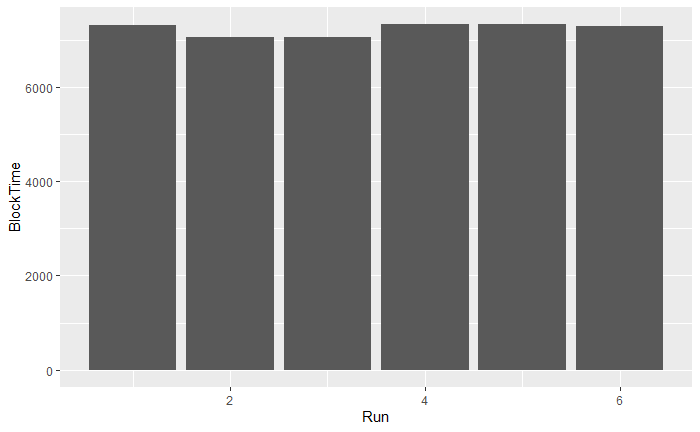
\includegraphics[scale=0.33]{./graph/Perc10_Block.png}
	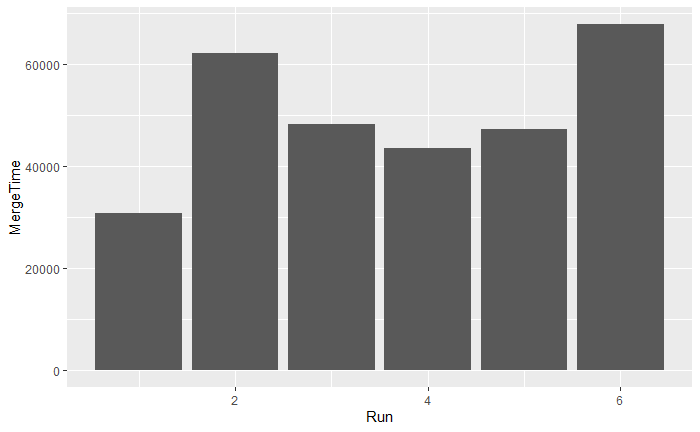
\includegraphics[scale=0.33]{./graph/Perc10_Merge.png}
	\item The 50\% file size was run three times. The completion times were ranging from 74740.1ms for the lowest and 140552ms for the highest time required to sort the blocks. To be noted for the highest time, a different process writing to file was occurring during the testing, which might have slowed the algorithm down to a degree, since they were writing onto the same drive, but we don't want to take away the possibility of that not being the case. The amount of MergeJobs, or amount of rounds to merge blocks, was 1504. 1514 if you consider the tasks of cleaning up the data and flushing it, which was also consistent throughout. The time required to merge was ranging from 1.38534e+06ms as the fastest time recorded in our experiment runs and 1.49018e+06ms as the highest.\\
	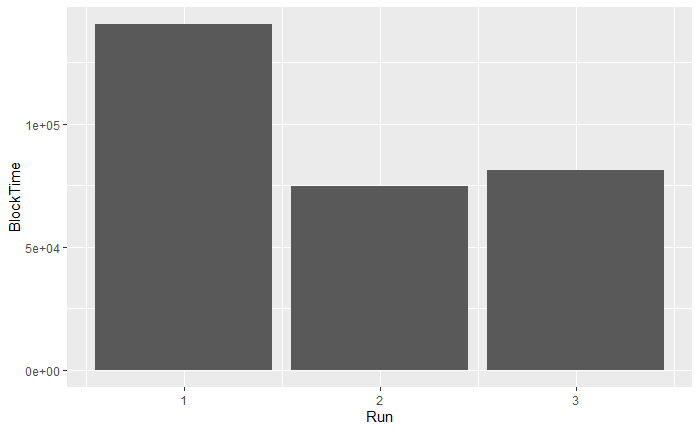
\includegraphics[scale=0.33]{./graph/Perc50_Block.png}
	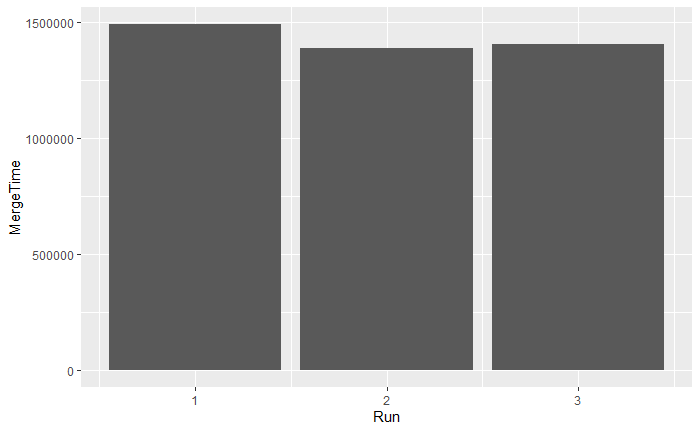
\includegraphics[scale=0.33]{./graph/Perc50_Merge.png}
	\item The 100\% file was tested once, due to time constraints. The completion time for the block sorting was 170696ms, with the amount of rounds being 3005, with clean jobs included a total amount of 3016. Merging was completed after 3.06425e+06ms.
	\item The 1,000\% file wasn't tested due to memory storage issues that would occur from running it on the described test machine. Further discussion regarding this will be held in the following section, regarding this file, but the other files as well.
\end{itemize}
\newpage
\section{Discussion and Conclusion}
As was seen with the results of the smaller sizes, the algorithm worked well with a fine time. The larger files proved to be problem on the device used for testing, which resulted in quite a long time needed for the merging process. After we completed our test runs on the described device, we tested it on another system, with higher or rather newer hardware and we were able to see a stark difference in performance. As a main example, the 100\% file, which took 3.06425e+06ms to complete the merging process in our previous runs, the other device managed to merge them in 122653ms. This contrast in time required can also be translated to the other data sizes.\\
Following this, we raise the assumption that this discrepancy is due to I/O operations being limited on the used device and a potential degeneration of hardware also manifesting over time, leading to needing much more time to complete all operations. But also a difference in the CPU used can be a different kind of bottleneck, due to the speed of operations, but also how much it can hold and change its cache.\\
Due to timing constraints we weren't able to use the new device for testing, but we think it would prove better times for the algorithm as the one we presented here. If possible, these should be seen as the worst-case times, that can occur due to hardware limitations.\\

To conclude this report, while the times recorded were biased in regards to being slowed down due to suspected hardware limitations and degeneration, which were discovered after testing, the algorithm itself works as intended and is expected to perform better than the times presented here on other hardware than the described one above.



\end{document}
